\chapter[Resultados]{Experimentos e Resultados}
\label{resultados}
Nessa seção, detalhes dos experimentos realizados, bem como resultados experimentais são mostrados a partir de simulações utilizando as bases de dados apresentadas na \secref{metodologia}. Como forma de avaliação são consideradas as taxas de acertos, de falsos positivos e negativos. Em outras palavras, os \textit{datasets} avaliados possuem arquivos de respostas, onde os tráfegos normais e ataques são descriminados. Assim, a resposta do \textit{framework} estudado será comparada com esse arquivo e a taxa de acertos será calculada da seguinte forma
\begin{equation}
	T_a = \left(1 - \frac{N_e}{N_t}\right)* 100,
\end{equation}
onde $T_a$ é a taxa de acertos, $N_e$ é o número tráfegos julgados erroneamente, $N_t$ é o número de tráfegos analisados pelo \textit{framework}. Além disso, as taxas de falsos positivos e negativos tem formulação semelhante.

\section{Análise \textit{dataset}\cite{DataMining}}  
Na \figref{fig:ResultsMining} tem-se os gráficos de taxa e acerto em função dos diferentes limiares simulados para o \textit{dataset} proposto por \cite{DataMining}, o qual possui apenas ataques e da forma como foi descrito na \secref{metodologia}. Para valores de limiar entre 0.8 e 0.84 a taxa de acerto permanece acima de 98.4\% e conforme o aumento do limiar, a taxa de acerto vai decrescendo. Tal comportamento é esperado, visto que para valores altos de limiar, o tráfego analisado deve ter propriedades (entropia, variação de IPs origem e taxa de pacotes) muito próximas do perfil normal para não ser considerado um ataque. Desta forma, vale ressaltar que existem diferentes tipos de ataques DDoS e geralmente possuem abordagens singulares para os ataques. Assim, seria uma escolha equivocada escolher valores de limiar próximos a 1, pois a granularidade dos ataques não seria abrangida pelo \textit{framework}. A \tabref{Tab:ResultsMining} complementa o gráfico da \figref{fig:ResultsMining}, pois mostra o número de acertos, falsos positivos e falsos negativos na análise do \textit{dataset}.

 \begin{figure}[htb]
 	\centering
 	\caption{Análise do \textit{dataset} avaliado }
 	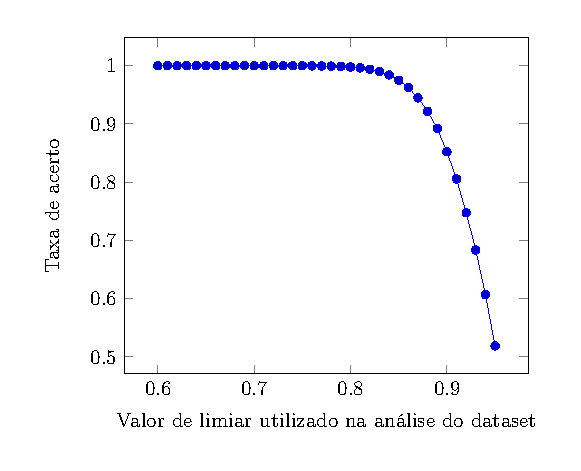
\includegraphics[width=0.7\textwidth]{figs/results80-95Mining.pdf}\\
 	{Fonte: Elaborada pelo autor.}
 	\label{fig:ResultsMining}
 \end{figure}
 
 \begin{table}[htb]
 	\centering
 	\begin{threeparttable}
 		\caption{Exemplo base de dados DARPA}
 		\label{Tab:ResultsMining}
 		%	\small
 		\begin{tabular}{c c c c}
 			\toprule
 			\textbf{Limiar} & \textbf{Taxa de acerto} & \textbf{Taxa de falsos positivos} & \textbf{Taxa de falsos negativos}
 			\\ \midrule
 			0.80 &  99.7790\% &  0\%& 0.2210\%   \\ \midrule
 			0.82 &  99.3905\% & 0\% & 0.6095 \%   \\ \midrule
 			0.84 &  98.4137\%  & 0\% & 1.5863\%   \\ \midrule
 			0.86 &  96.2556\%  &  0\% & 3.7444\%   \\ \midrule
 			0.88 &  92.1842\%  &  0\% & 7.8158\%     \\ \midrule
 			0.90 &  85.2309\%  & 0\% & 14.7691\%    \\ \midrule
 			0.92 &  74.7722\%  &  0\% & 25.2278\%   \\ \midrule
 			0.94 &  60.6753\%  & 0\% & 39.3247\%   \\ \bottomrule
 		\end{tabular}
 		{Fonte: Elaborada pelo autor.}
 	\end{threeparttable}
 \end{table}
 Note que a coluna da taxa de falsos positivos consta com $0\%$ devido a natureza do \textit{dataset} ser apenas de ataques. Logo, não é possível o \textit{framework} detectar um tráfego como ataque e ele na realidade ser um fluxo normal. Por outro lado, é possível detectar um tráfego como normal, sendo que ele trata-se de um ataque, como mostrado na tabela.
\section{Análise \textit{dataset} DARPA}
A \figref{ass} apresenta os gráficos da taxa de acertos em função dos limiares simulados 



   